\chapter{図と式}\label{chap:method}

\section{図の入れ方}
図のファイルは figures フォルダーに入れます。
\figref{fig:sample}のように、図の番号は章ごとに付き、キャプションは図の下に置きます。

\begin{figure}[htbp]
  \centering
  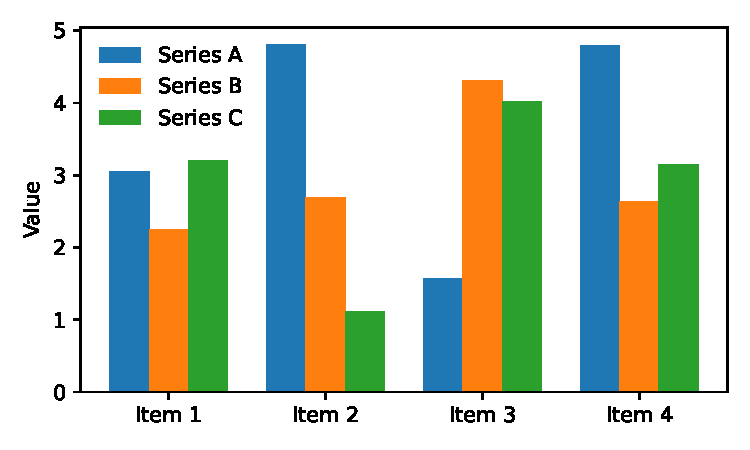
\includegraphics[width=0.7\linewidth]{figures/sample-chart.pdf}
  \caption{棒グラフの例}\label{fig:sample}
  \source{著者による}
\end{figure}

\section{式の書き方}
番号の付いた式は \verb|equation| 環境で書きます。
\eqref{eq:sample}のように、本文から式を参照できます。
\begin{equation}
  F(x) = \int_{0}^{1} x^{2} \, dx
  \label{eq:sample}
\end{equation}
